%%+++++++++++++++++++++++++++++++++++++%%
%%         Final Version  6/14/95      %%
%%+++++++++++++++++++++++++++++++++++++%%
\documentclass[12pt]{article}
\textheight = 8.6in
\textwidth = 6.2in
\topmargin = -.5in
\oddsidemargin = 0.08in
\evensidemargin = 0.08in
%\usepackage{fancyhdr}
%\pagestyle{fancy}
%\rfoot{\thepage}
\setlength{\jot}{10.0 pt}
\setlength{\parskip}{2.0ex}
\setlength{\footskip}{65pt}

\usepackage{graphicx}
\usepackage{subfigure}
\usepackage{placeins}
\usepackage{afterpage}
\usepackage{amsmath}
\usepackage{empheq}
\usepackage[most]{tcolorbox}
\newtcbox{\mymath}[1][]{%
    nobeforeafter, math upper, tcbox raise base,
    enhanced, colframe=white!20!black ,
    colback=blue!30!red!30!white, boxrule=1pt,
    #1}
\usepackage{xcolor}
\definecolor{myblue}{RGB}{0, 0, 180}   %Numbers are integers from 0 to 255, smaller is closer to black


\begin{document}

\begin{flushright} {\color{blue} Chapter 2, Lecture 4} \end{flushright}
\begin{flushleft}

\subsubsection*{\bf Conductors}

Conductors are materials in which electrons are free to move through the material.  Metals are usually conductors.  The atoms in a material bond in a crystalline structure (see Fig.~\ref{fig:culattice}).  

\begin{figure}[h]
\centering
\includegraphics*[trim=0cm 4cm 1cm 2cm, clip=true, width=0.6\columnwidth]{Cu_lattice.pdf}
\caption{\small Copper lattice from two perspectives, coutesy Dr. Karoly Nemeth.}
\label{fig:culattice}
\end{figure}

When electrons are bound to a single atom, they are trapped in the potential well of the nucleus.  There are distinct allowed energy levels as shown in Fig.~\ref{fig:wells}.  When atoms form a crystal structure the potential barrier between adjacent atoms is lowered, allowing electrons with high enough energy to delocalize.  An energy band with energy greater than the height of the potential barrier extends through the crystal, allowing electrons in the band to move freely through the crystal. 

\begin{figure}[h]
\centering
\includegraphics*[trim=0cm 0cm 0cm 0cm, clip=true, width=0.6\columnwidth]{wells.png}
\caption{\small Cartoon of a potential well with electron energy levels for a single atom (left) and potential wells with electron energy bands in a metal (right).}
\label{fig:wells}
\end{figure}

\subsubsection*{\bf Fields and potentials of conductors}

Once a conductor is in static equilibrium (electrostatic regime) all excess charge resides on the surface(s) of the conductor, and the electric field {\it is zero} inside the conductor.  Suppose that some charges were inside the conductor; they would create electric fields in the conductor, and these would push the charges around and create currents.  If this persisted, then there would be perpetual currents that violate conservation of energy.  When there are no charges inside a conductor, Gauss' law verifies that there cannot be an electric field inside either.  Consider the conductor sketched in Fig.~\ref{fig:empty}, with a Gaussian surface placed just inside the actual surface.

\begin{figure}[h]
\centering
\includegraphics*[trim=0cm 1cm 0cm 1cm, clip=true, width=0.6\columnwidth]{gsurface.png}
\caption{\small Gaussian surface just inside the surface of an arbitrarily shaped conductor.}
\label{fig:empty}
\end{figure}

Gauss' law is given by:
\begin{equation}
\oint_{S} \vec{E} \cdot d\vec{a} = \frac{q_{enc}}{\varepsilon_{0}} 
\label{eq:glaw}
\end{equation}

There is no charge inside the Gaussian surface, $q_{enc}=0$, so the RHS of Eq.~\ref{eq:glaw} is zero.  This then requires that the LHS also be zero.  The only way for this to always be true is to have $\vec{E}=0$ at the Gaussian surface.  This argument holds for any choice of Gaussian surface inside the conductor, so the conclusion is that there is no electric field inside a conductor. 

The electric field produced by the excess charge on the surface of a conductor must be perpendicular to the surface everywhere.  If there were a tangential component of the electric field along the surface, it would push charges around on the surface, again creating currents in violation of conservation of energy.  If a conductor is surrounded by an insulator (such as air), when the field is only in the perpendicular direction, the charges cannot move.  They cannot migrate off the conductor since there is no path for the charge through the surrounding insulator.

\begin{figure}[h]
\centering
\includegraphics*[trim=0cm 0cm 0cm 0cm, clip=true, width=0.5\columnwidth]{fieldlines.png}
\caption{\small Electric field lines are perpendicular to the surface of a conductor.}
\label{fig:wequip}
\end{figure}

Since there is no tangential component of the electric field along the surface of a conductor, the surface of a conductor is an {\color{myblue} {\it equipotential surface}}.  It has been shown previously that $\vec{E}=-\vec{\nabla}V$, implying that the field points in the direction of maximum change of the potential.  If $\Delta E=0$ along a surface, then the 3D slope of the potential is zero along the surface, and the potential itself must be constant.  The equipotential surfaces around a conductor will mimic the surface of the conductor, since they are normal to the field direction everywhere.  Some equipotential surfaces are sketched in Fig.~\ref{fig:wequip}, along with the field lines.

\vspace{.2in}
\begin{figure}[h]
\centering
\includegraphics*[trim=0cm 0cm 0cm 0cm, clip=true, width=0.6\columnwidth]{and_equipotentials.png}
\caption{\small Now the equipotentials lines are also shown.}
\label{fig:wequip}
\end{figure}

\subsubsection*{\bf The advantage of being `well-rounded'}

The Feynman lectures have a nice discussion about how an electric field is strongest at the sharpest points (smallest radiuses of curvature) of a conductor.  The electric field is larger there because the charge density is larger.  Charge collects more on corners, protrusions and points.  For this reason, a conductor on high voltage equipment is as smooth and rounded as possible (c.f. Fig.~\ref{fig:cwagain} which shows the -750 kV Cockroft-Walton DC accelerator).

\begin{figure}[h]
\centering
\includegraphics*[trim=0cm 2cm 0cm 0cm, clip=true, width=0.7\columnwidth]{cwagain.pdf}
\caption{\small Left: the historical Fermilab Cockroft-Walton -750 kV DC accelerator ({\it Courtesy Fermilab visual media services}).  Right: Lightning is an example of arcing due to build up of static charge ({\it Courtesy NOAA Photo Library, Photgrapher C. Clark}).}
\label{fig:cwagain}
\end{figure}

Feynman used a simple model to demonstrate the field enhancement near small radiuses of curvature; it  consists of a large spherical conductor connected by a long thin conducting wire to a small spherical conductor (see Fig.~\ref{fig:round}).  The two spheres and connecting wire are all one equipotential conducting surface, but the wire is taken to be long enough that the field near the surface of a given sphere is well approximated by the field due to that sphere alone. 

\begin{figure}[h]
\centering
\includegraphics*[trim=0cm 0cm 0cm 0cm, clip=true, width=0.4\columnwidth]{vspheres.pdf}
\caption{\small An equipotential object with a large and a small sphere connected by a wire.}
\label{fig:round}
\end{figure}

So, the magnitude of the field near the large sphere of radius $R$ is $E=\frac{Q}{4\pi\varepsilon_{0}R^{2}}$, where $Q$ is the charge on the large sphere.  The magnitude of the field near the small sphere of radius $r$ is $E=\frac{q}{4\pi\varepsilon_{0}r^{2}}$, where $q$ is the charge on the small sphere.  Then, taking the ratio of the field at the surface of the small sphere to the field at the surface of the large sphere, 

\begin{equation}
\frac{E_{small}}{E_{large}} = \frac{\left(\frac{q}{4\pi\varepsilon_{0}r^{2}}\right)}{\left( \frac{Q}{4\pi\varepsilon_{0}R^{2}} \right)}
=\frac{ qR^{2} }{ Qr^{2} }
\label{eq:eratio}
\end{equation}  

Since it is all one conductor, the potential at the surface of the small sphere must be the same as the potential at the surface of the large sphere,

\begin{eqnarray}
V_{small} & = & V_{large} \nonumber \\
\frac{Q}{4\pi\varepsilon_{0}R} & = & \frac{q}{4\pi\varepsilon_{0}r} \nonumber \\
\frac{Q}{R} & = & \frac{q}{r} \label{eq:qor}
\end{eqnarray}

Equation~\ref{eq:qor} enables cancellation in Eq.~\ref{eq:eratio}, with the result that the ratio of the fields at the surface of the spherical conductors is inversely proportional to their radii of curvature.

\begin{equation*}
\frac{E_{small}}{E_{large}} =\frac{ R }{ r }
\end{equation*}  

Consider the accelerating column shown in Fig.~\ref{fig:cwagain}; it is desirable to have a very large accelerating field in the column so that it can be as short as possible.  The work done on a charge $q$ in a uniform field is $W=\Delta \mbox{KE}= qEL$, where $L$ is the length of the accelerating column.  If the column length $L$ is made shorter, then to get the same change in kinetic energy, the electric field must become correspondingly larger.  In order to produce a larger field, there must be more charge on the electrodes.  At some point, the density of static charge becomes so high that it cannot be maintained and electrical `breakdown' (arcing of electric current) will occur.  The electric field near the conductor becomes large enough that it ionizes the air nearby, the ion path extends, eventually making it from the conductor to ground.  At that point, there is a completed circuit, and charge flows (suddenly) along the ionization path.  This is the same mechanism responsible for lightning.  In general, most types of accelerating structures in particle accelerators are metallic (either normal or superconducting) and since it is desirable for the magnitude of the electric fields inside be as high as possible, great care is taken to make sure the metallic surfaces are as smooth and free of imperfections as possible.


\subsubsection*{\bf Coaxial cable}

The coaxial cable is a very useful arrangement of conductors.  A dissected view of a typical coaxial cable is shown in Fig.~\ref{fig:coaxcable}.

\begin{figure}[h]
\centering
\includegraphics*[trim=0cm 1cm 0cm 2cm, clip=true, width=0.6\columnwidth]{coax_dissect.pdf}
\caption{\small The inside of a coaxial cable.  This image from\\ http://www.cablewholesale.com/support/technical\_articles/coaxial\_cable.html.}
\label{fig:coaxcable}
\end{figure}

The figure shows the center conductor (wire) surrounded by a dielectric (insulator), with an outer shield that is essentially a conducting shell surrounding the inner conductor.  There is an insulating jacket surrounding the shield.  A schematic of the electrical hook-up is shown in Fig.~\ref{fig:coaxschematic}. 

\begin{figure}[h]
\centering
\includegraphics*[trim=0cm 2cm 0cm 3cm, clip=true, width=0.6\columnwidth]{coax_schematic.pdf}
\caption{\small A schematic of a circuit with coaxial cable.  This image from\\ 
http://en.wikipedia.org/wiki/File:Transmission\_line\_schematic.svg.}
\label{fig:coaxschematic}
\end{figure}

 The hot side of the power source is connected to the central conductor of the coax and carries current to the load (denoted $Z_{L}$ in the figure).  The return path for the current is the outer conductor (shield), which is normally connected to ground.
 
Since we are still in the electrostatics zone, consider the coax geometry but instead of having a current run along the central conductor, have a static line density of charge, $\lambda_{in}=\lambda$.  Let the outer conductor have an equal and opposite linear charge density, $\lambda_{out}=-\lambda$.  Let the cylindrical conductors be infinitely long so that the situation can be analyzed using Gauss' law.  The geometry is shown in Fig.~\ref{fig:coax2}; the radius of the inner conductor is $a$, and the radius of the outer conductor is $b$.
% note to self, use coaxcyl.png but must go change I to lambda

\begin{figure}[h]
\centering
\includegraphics*[trim=0cm 0cm 0cm 0cm, clip=true, width=0.6\columnwidth]{coax2.png}
\caption{\small Side view and cross-sectional view of a coaxial cable with center conductor of radius $a$ and outer conductor of radius $b$.  Also shown is a Gaussian surface (a short cylinder of length $\Delta l$) that can be used to find the field at $a<s<b$.  In the cross-sectional view, the dashed circle represents the end of the Gaussian surface.}
\label{fig:coax2}
\end{figure}

The electric field is zero at $s<a$ since the inner cylinder is conducting.  In order to find the electric field in the region where $a<s<b$, put a cylindrical Gaussian surface at $s$ with ($a<s<b$), and concentric with the central axis (the $z$-axis of the cylindrical coordinate system).  Only the change enclosed by the Gaussian surface contributes to the field at the surface.  The total charge enclosed by the Gaussian surface of length $\Delta l$ is given by,

\begin{equation}
Q_{in}=\lambda \; \Delta l
\label{eq:coaxcharge}
\end{equation}

The shell theorem says that the field is the same as it would be from a line charge with charge density $\lambda$ lying along the axis of symmetry.  Anyway, the symmetry of the geometry guarantees that the electric field from the inner conductor points in the $\hat{s}$ direction everywhere, and that the field can only depend on the $s$ coordinate, not $\phi$ or $z$.  This makes the flux integral particularly easy to calculate:
\begin{eqnarray}
\oint \vec{E} \cdot d\vec{a} & = & \int_{barrel} \hspace{-.2in} E\hat{s} \cdot\hat{s} da + \int_{endcap1} \hspace{-.3in} E\hat{s} \cdot -\hat{z} da + \int_{endcap2} \hspace{-.3in} E\hat{s} \cdot \hat{z} da \nonumber \\
\vspace{.1in}
 & = & E\int_{barrel} \hspace{-.2in} da \hspace{.1in} + \: 0 \: + \:0 \nonumber\\
 \vspace{.2in}
 & = & E (2\pi s) \Delta l 
\label{eq:coaxflux}
\end{eqnarray}

Combining the results of the flux calculation (Eq.\ref{eq:coaxflux}) with the charge calculation (Eq.\ref{eq:coaxcharge}, Gauss' law may be solved for the electric field between the two conductors:
\begin{eqnarray}
\oint \vec{E} \cdot d\vec{a} & = & \frac{Q_{in}}{\varepsilon_{0}} \nonumber \\
 E\int_{barrel} \hspace{-.2in} da & =  &  \frac{\lambda \; \Delta l}{\varepsilon_{0}} \nonumber \\
E (2\pi s) \Delta l  & = & \frac{\lambda \; \Delta l}{\varepsilon_{0}} \nonumber \\
E & =& \frac{\lambda}{2\pi \varepsilon_{0} s}
\label{eq:what?}
\end{eqnarray}

The next region to consider is where $r>b$.  Now the Gaussian surface must be outside both conductors, as shown in Fig.~\ref{fig:coaxout}.

\begin{figure}[h]
\centering
\includegraphics*[trim=0cm 0cm 0cm 0cm, clip=true, width=0.6\columnwidth]{coax1.png}
\caption{\small Side view of a coaxial cable with center conductor of radius $a$ and outer conductor of radius $b$.  Also shown is a Gaussian surface (a short cylinder of length $\Delta l$) that can be used to find the field at $s>b$.}
\label{fig:coaxout}
\end{figure}

In order to find the electric field in the region where $s>b$, put a cylindrical Gaussian surface at $s$ with ($s>b$), and concentric with the central axis (the $z$-axis of the cylindrical coordinate system).  Only the change enclosed by the Gaussian surface contributes to the field at the surface.  Now the total charge enclosed by the Gaussian surface is zero,

\begin{equation*}
Q_{in}=\lambda \; \Delta l -\lambda \; \Delta l = (\lambda - \lambda) \Delta l = 0
\end{equation*}

The shell theorem says that the field is the same as it would be from a line charge with charge density $\lambda$ lying along the axis of symmetry, and a line charge with charge density $-\lambda$ also lying along the axis of symmetry.  The net enclosed charge is zero, so the flux integral must also be zero.  Gauss' law tells us that there is no electric field outside the coaxial cable.  That is one reason people use this type of cable; coaxial cables don't `leak' field into their surrounding environment.

\subsubsection*{\bf Faraday cage}

If there are other charges and fields outside the conductor, the charge on the conductor will move to screen the external electric field from the interior of the conductor.  This is the principle behind a Faraday cage or Faraday shield.  A Faraday cage or shield is a field-free enclosure made so by using conducting outer walls.  These are sometimes used to shield sensitive electronics.  This is also the basic idea of the `drift tubes' in an accelerating structure for a particle accelerator.

%Drift tubes.\\
\iffalse
\begin{figure}[h]
\centering
\subfigure[Conductor]
{\label{fig:total}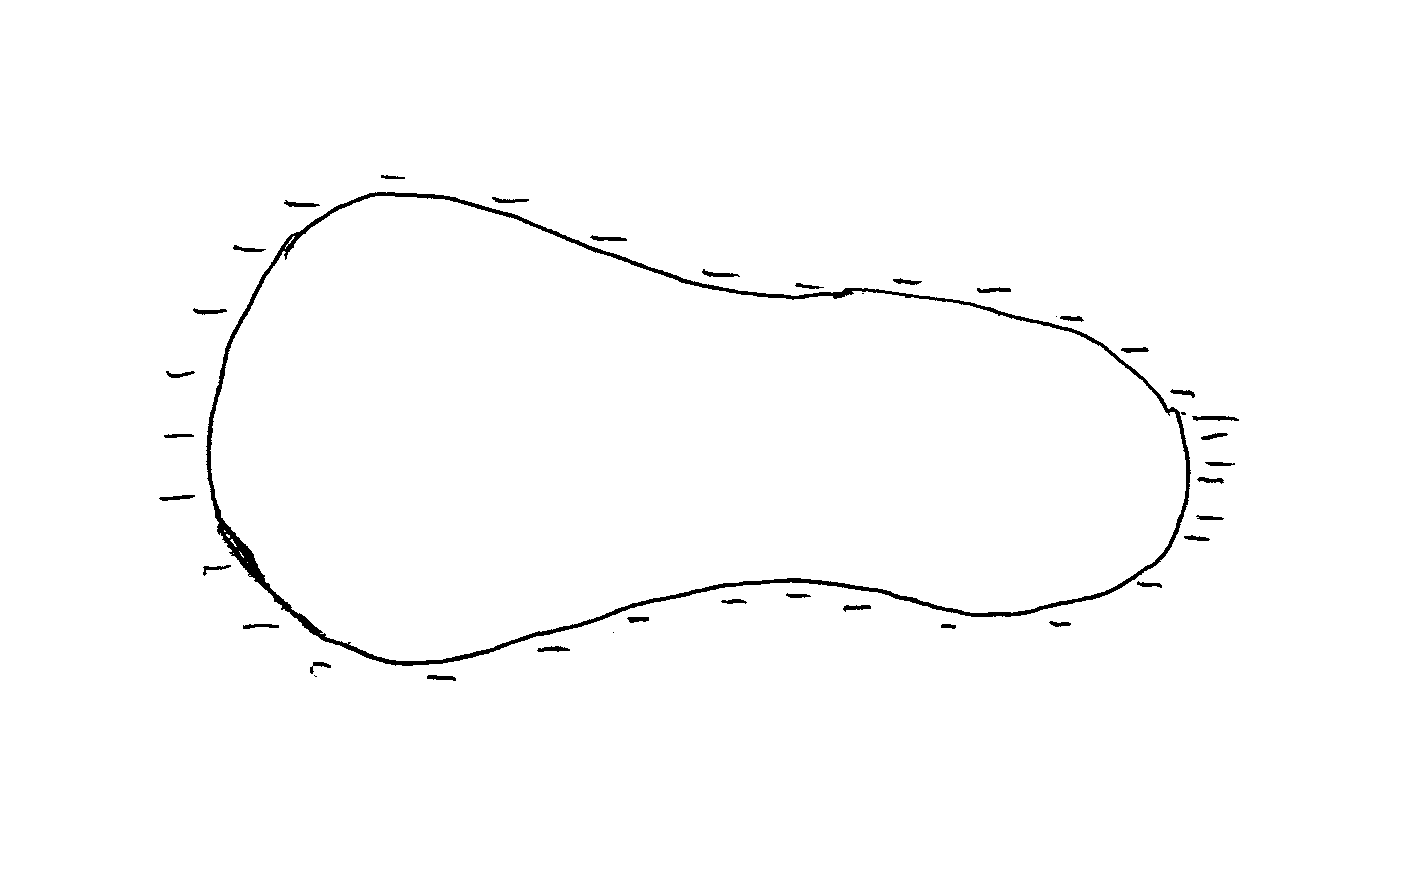
\includegraphics[width=.40\columnwidth]{silly_conductor.png}}
%\hspace{.1in}
\subfigure[Conductor and field lines]
{\label{fig:onesig}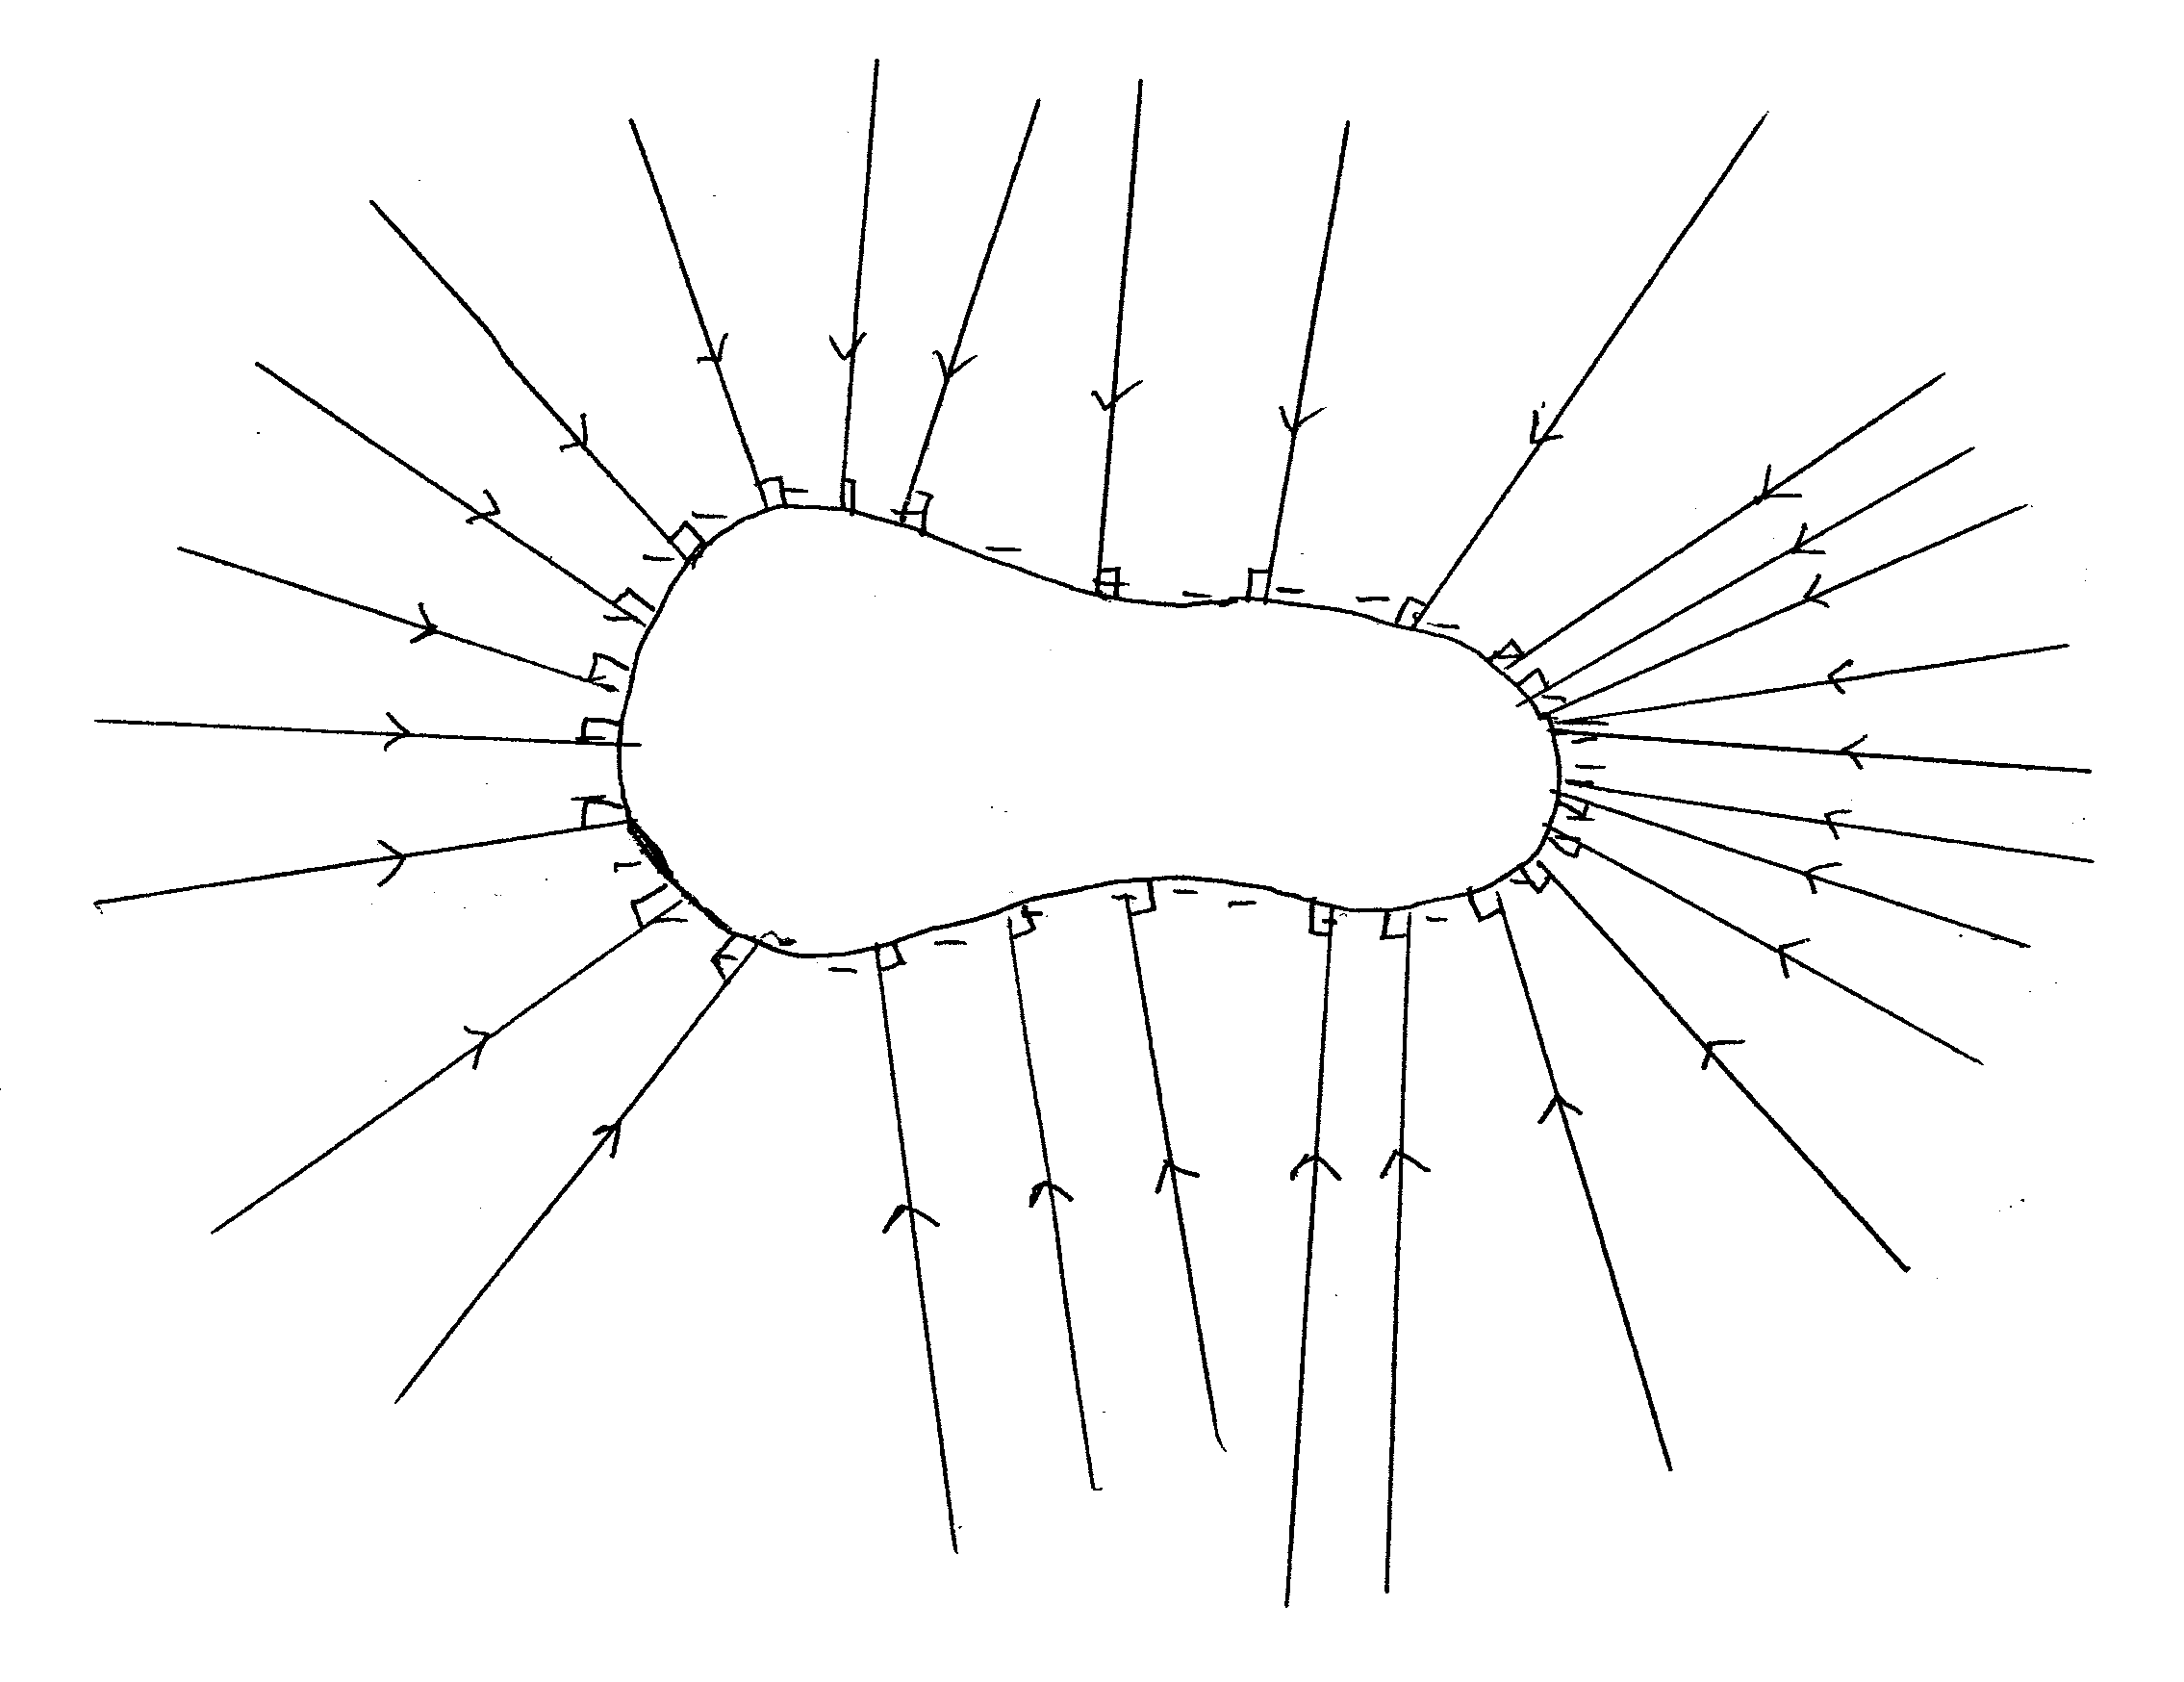
\includegraphics[width=.55\columnwidth]{fieldlines.png}}
\caption{The left subfigure shows a conductor with excess charge that is all on the surface.  The right subfigure shows the same conductor and the field lines produced by the excess charge.  The conductor surface is an equipotential surface, and the field lines terminate at right angles to the surface.}
\label{fig:conductor}
\end{figure}
\fi



\end{flushleft}
\end{document}








